\section{Como a Máquina Aprende}
\label{sec:howdoesmachinelearn}

O processo básico de aprendizagem de máquina consiste em entrada de dados, abstração e generalização.
\begin{alineas}
	\item Entrada de dados: são fatos tirados da memoria ou da observação;
	\item Abstração: transformar estes dados em algo mais objetivo e que faça sentido;
	\item Generalização: utiliza os dados abstraídos e para  identificar padrões e assim classifica-los;			
\end{alineas}

\begin{figure}[h!]
	\centering
	\Caption{\label{fig:processo-aprendizagem} Fluxo do processo de aprendizagem.}	
	\UECEfig{}{
		\fbox{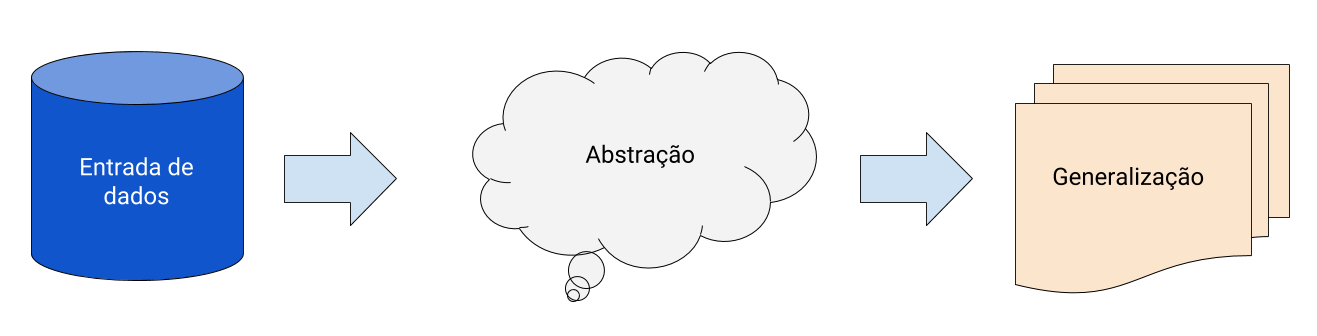
\includegraphics[width=15cm]{figuras/procc-learning}}
	}{
		\Fonte{Elaborado pelo autor}
	}	
\end{figure}

Todo este processo ocorre na ordem apresentada, pois o conceito de abstração e generalização estão muito próximos e tecnicamente um não faz sentido sem o outro. Os passos de abstração e generalização do processo de aprendizagem ocorrem subconscientemente em seres humanos, logo pode ser complexo representar este processo em linguagem computacional.


\subsection{Abstração e Representação de Dados}
\label{cap:abs-representacao-dados}

Durante a abstração os dados de entradas, são preparados para que possuam algum sentido em um contexto.
Para ilustrar este processo, lembre de quando aprendeu a executar operações de soma e subtração, que sua professora apresentou o exemplo:

\begin{figure}[h!]
	\centering
	\Caption{\label{fig:exemplo-aprendizagem} Uma maçã mais outra maçã é igual à duas maçãs.}	
	\UECEfig{}{
		\fbox{
\includegraphics[width=15cm]{figuras/exemplo_soma_maca}}
	}{
		\Fonte{Elaborado pelo autor}
	}	
\end{figure}

Você ignorou todas as propriedades da maçã como ser uma fruta, ter a cor vermelha  ou possuir sementes, e focou nas propriedades que faziam sentido no contexto, que é a maçã representar uma unidade. Logo uma unidade de um tipo mais outra unidade do mesmo tipo é igual à duas unidades, ou seja para o contexto de soma não importa se é uma fruta ou a cor e sim a unidade. Após o processo de abstração formou-se a seguinte ideia:


\begin{figure}[h!]
	\centering
	\Caption{\label{fig:exemplo-aprendizagem} Exemplo soma com maçãs após o processo de abstração.}	
	\UECEfig{}{
		\fbox{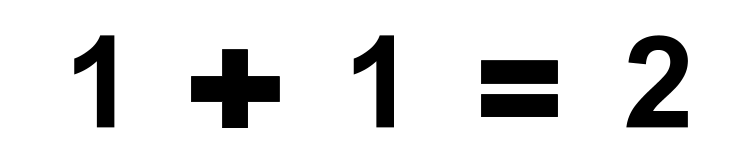
\includegraphics[width=15cm]{figuras/exemplo_soma_maca2}}
	}{
		\Fonte{Elaborado pelo autor}
	}	
\end{figure}

A etapa seguinte do processo de abstração é a representação do conhecimento, onde é gerado um 
\textbf{\textit{modelo}}\footnote{Modelo é uma representação explícita dos padrões encontrados entre os dados.}. 
Existem vários tipos de modelos, alguns deles são:
\begin{alineascomponto}
    \item Equações;
    \item Grafos;
    \item Estruturas de logicas de programação como: \textit{if} e \textit{else}; 
\end{alineascomponto} 

A escolha do modelo não é feita pelo sitema de aprendizagem, depende do tipo da tarefa \textbf{\textit{T}} e o tipo dos dados
que estão sendo analisados. A etapa que gera um modelo específico de um conjunto de dados é chamada de treino do modelo \textbf{\textit{E}}. 
Quando um modelo é treinado, os dados são transformado em uma forma abstrata que resume os dados originais, é importante observar que o  
treino do modelo não gera novos dados, muitas vezes após esta etapa nos surpreendemos com as teorias levantas sobre como 
estes dados se relacionam. Estas relações identificadas sempre estiveram presente, porém quando organizamos estes dados de outra forma
é possível identificar estas conexões escondidas.

\subsection{Generalização}
\label{cap:generalização-dados}

Até que o sistema possa utilizar o cohecimento abstrato para uma ação futura, o processo de aprendizagem ainda não está concluído.
O processo de generalização transforma o conhecimento abstrato prévio em um formato que possa ser utilizado para um ação, é um 
processo difícil de ser descrito, mas pode ser visto como uma busca nos modelos ou teorias geradas no processo de abstração, porém pode existir
um grande número de modelos disponíveis.

Dado que exista um grande número de teorias, durante a generalização este número será reduzido de forma qualitativa. 
Mas não é praticável examinar cada uma das teorias e verificar se será util, portanto os algoritmos de machine learning utilizam 
técnicas de busca como heurística \footnote{\cite{heuristica}A pesquisa por heurísticas é uma pesquisa realizada por meio da quantificação de proximidade a um determinado objetivo. 
Diz-se que se tem uma boa (ou alta) heurística se o objecto de avaliação está muito próximo do objetivo; diz-se de má (ou baixa) 
heurística se o objeto avaliado estiver muito longe do objetivo. Etimologicamente a palavra heurística vem da palavra grega Heuriskein, que significa descobrir (e que deu origem também ao termo Eureca).} 
ou palpites para diminuir a área de busca para encontrar os modelos mais importantes. Porém como a heurística trabalha com proximidade, 
não há garantias de que  que os melhores modelos serão escolhidos, no entanto é impraticável realizar esta pesquisa sem utilizar está técnica.

A heurística aplicada em aprendizagem de máquina as vezes resulta em conclusões erradas, se estas conclusões constantemente 
forem imprecisas, é necessário incluir uma tendência no algoritmo, algo como um pré-conceito sobre oque ele procura. Por exemplo 
dado um algoritmo que identifica rostos em imagens, ele procura por dois circulos(os olhos) em cima da linha da boca, logo isto 
pode ser considerado uma tendência, que causara problemas ao tentar reconhecer um rosto com óculos, rostos de perfil, com tons 
de pele mais escuros ou outras caracteristicas que não compreendem o modelo. É possivel incluir têndencias para que o algoritmo de 
um peso maior para olhos claros ou rostos com barbas. Porém pode ser um desafio identificar qual caracteristica terá mais peso que 
a outra no modelo escolhido. Contudo estas tendências são um mal necessário.

\subsubsection{Avaliando o sucesso da aprendizagem}
\label{cap:avaliando-generalização-dados}
A última etapa da generalização é determinar o sucesso dos modelos, depois de treinado com os dados iniciais
o modelo é testado em novos dados e avaliado como o processo de generalização se comporta, é importante ter em mente que é extremamente raro
que o modelo atenda perfeitamente todos os casos imprevistos.
Um dos motivos para que um modelo não generalize perfeitamente todos os casos é chamado de ruído, ou variações não previstas nos dados.
Estes ruidos são causados por dados corrompidos, cálculos imprecisos ou até mesmo entrada de dados inconsistentes.









 